%presentation} declaration
\documentclass[10pt]{beamer}
\usetheme{metropolis}

%packages
%beamer stuff
\usepackage{appendixnumberbeamer}
\usepackage{booktabs}
\usepackage[scale=2]{ccicons}
\usepackage{pgfplots}
\usepgfplotslibrary{dateplot}
\usepackage{xspace}
%language
\usepackage[utf8]{inputenc}
%images
\usepackage{graphicx}
\usepackage{float}

%macros
\newcommand{\tit}[1]{\textit{#1}}
\newcommand{\tbf}[1]{\textbf{#1}}
\newcommand{\ttt}[1]{\texttt{#1}}

%title
\title{Attention as a Leverage for Deep Learning}
\subtitle{}
\author{Erik Perillo\\
Advisor: Profa. Dra. Esther Colombini}
\date{\today}
\institute{Institute of Computing - Unicamp - Brazil}

\begin{document}

\maketitle

\begin{frame}{Outline}
    \begin{itemize}
        \item Introduction
        \item Background
        \item Methodology
        \item Work so far
    \end{itemize}
\end{frame}

\section{Introduction}

\begin{frame}{Introduction}
    \begin{figure}
        \centering
        
\includegraphics[width=1.0\linewidth]{./img/wheres_wally.jpg}
    \end{figure}
\end{frame}

\begin{frame}{Introduction}
    \begin{figure}
        \centering
        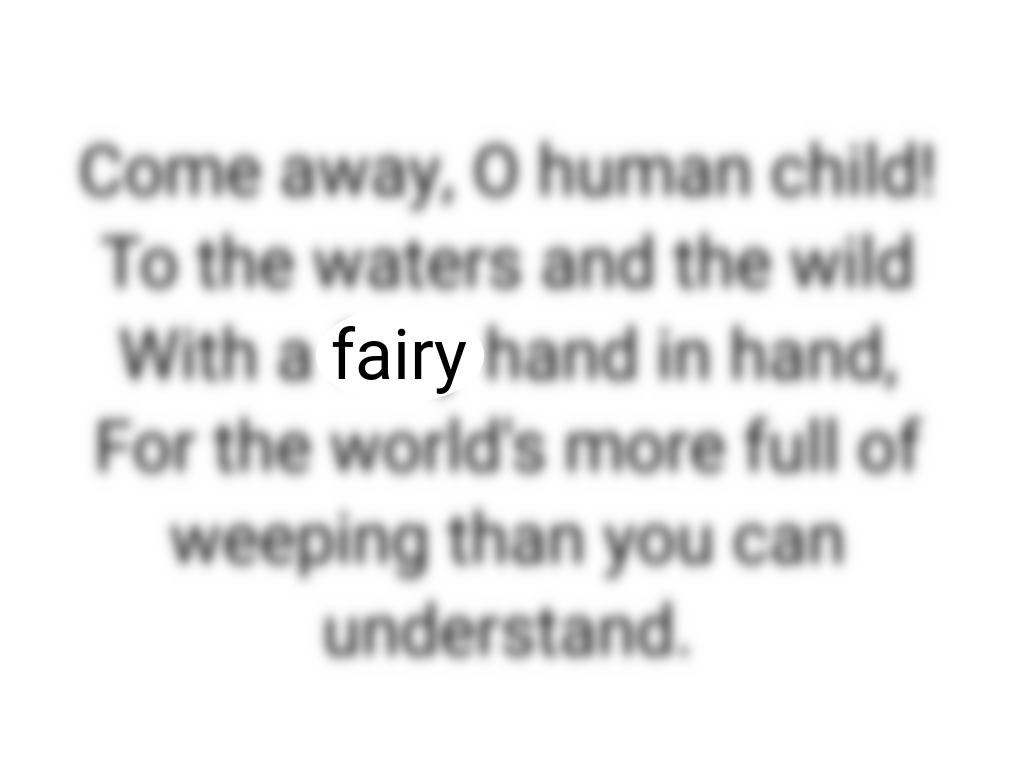
\includegraphics[width=1.0\linewidth]{./img/text_focus.png}
    \end{figure}
\end{frame}

\begin{frame}{Introduction}
    \begin{figure}
        \centering
        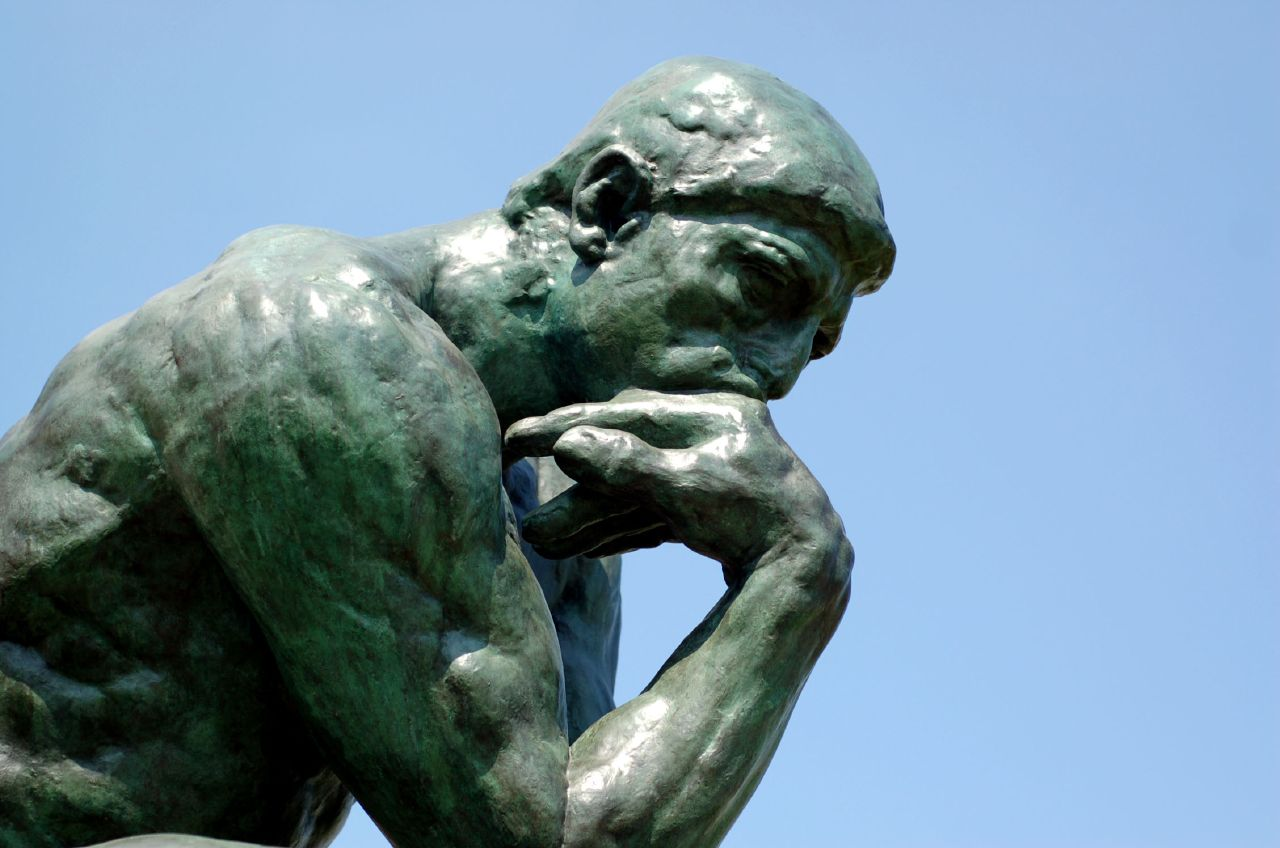
\includegraphics[width=1.0\linewidth]{./img/thinking.jpg}
    \end{figure}
\end{frame}

%\begin{frame}{Introduction}
%    \begin{figure}
%        \centering
%        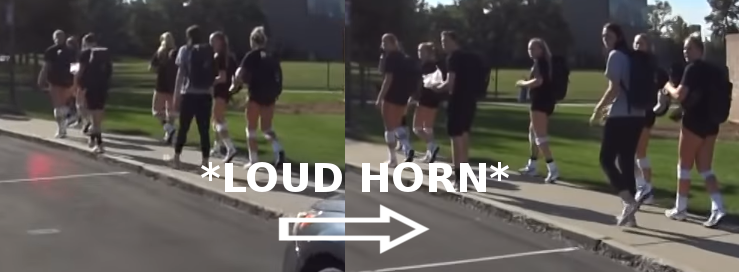
\includegraphics[width=1.0\linewidth]{./img/loud_horn.png}
%    \end{figure}
%\end{frame}

\begin{frame}{}
    \centering
    \textit{Attention: the ability to \textbf{filter and select} relevant stimuli,
        to \textbf{keep focus} on a task for an adequate amount of time.
        To appropriately \textbf{direct mental resources}}
\end{frame}

\begin{frame}{Attention for intelligence and AI}
    \begin{itemize}
        \item Fundamental for intelligence
        \item Fundamental for AI
    \end{itemize}
\end{frame}

\begin{frame}{The rise of Deep Learning}
    \begin{figure}
        \centering
        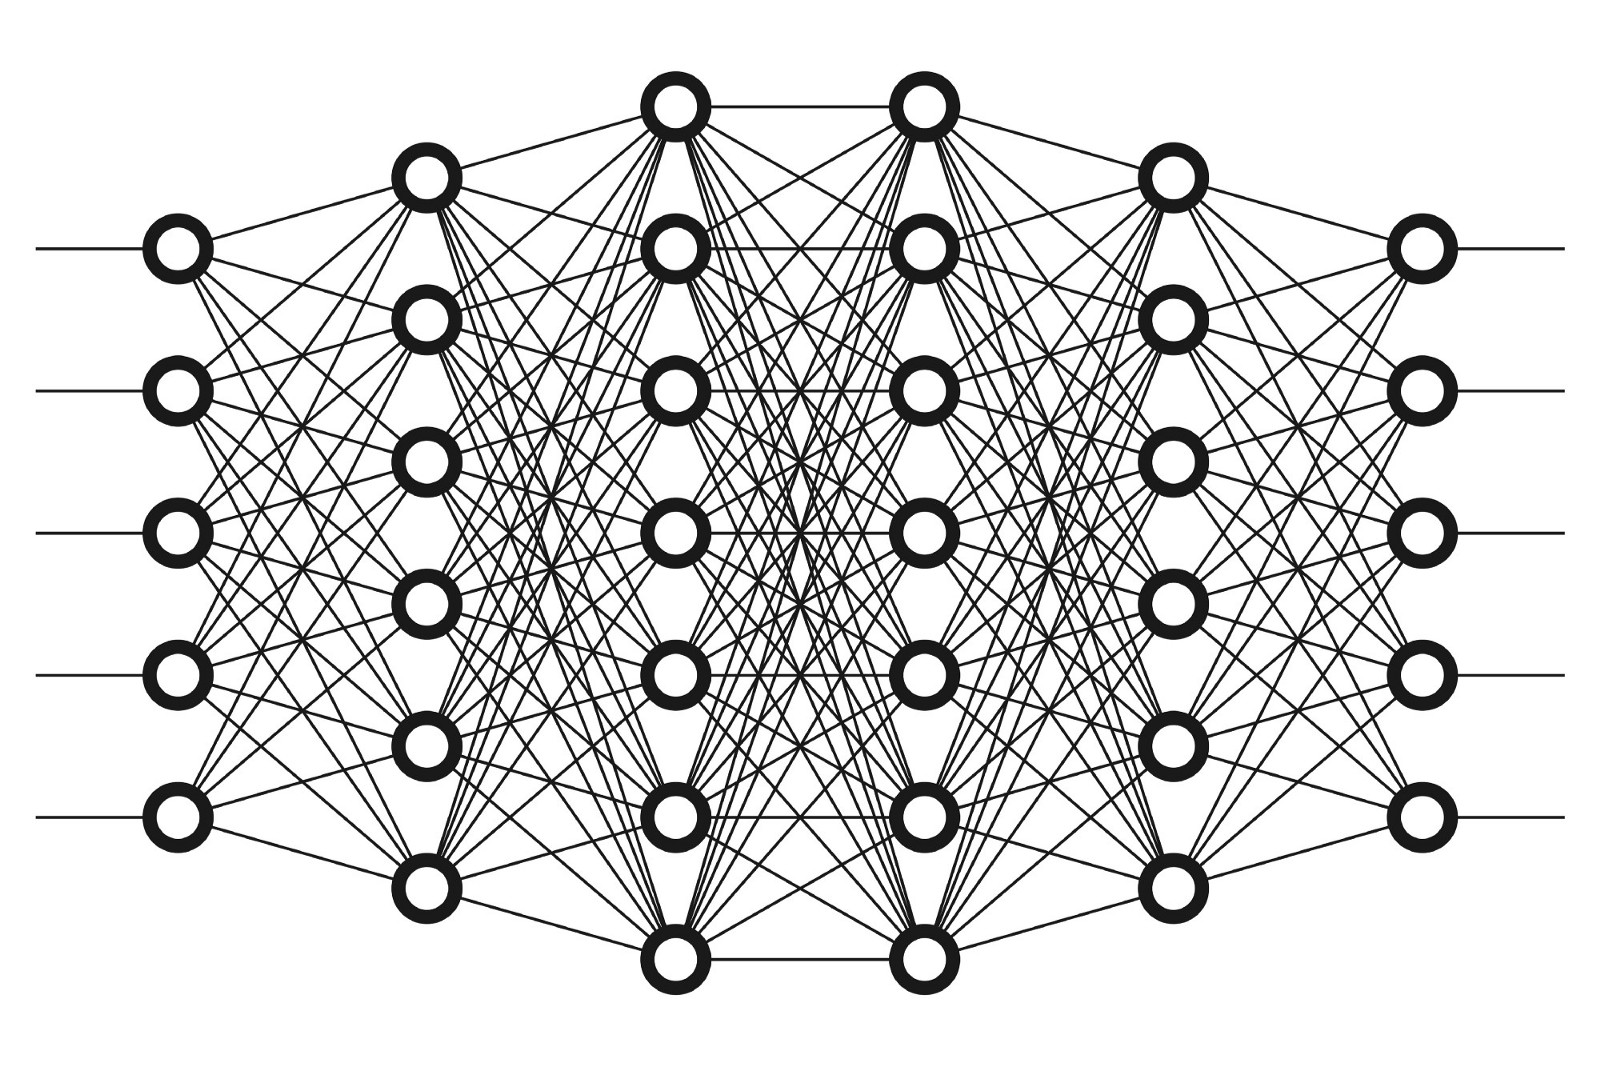
\includegraphics[width=1.0\linewidth]{./img/dl2.jpeg}
    \end{figure}
\end{frame}

%\begin{frame}{The rise of Deep Learning}
%    \begin{figure}
%        \centering
%        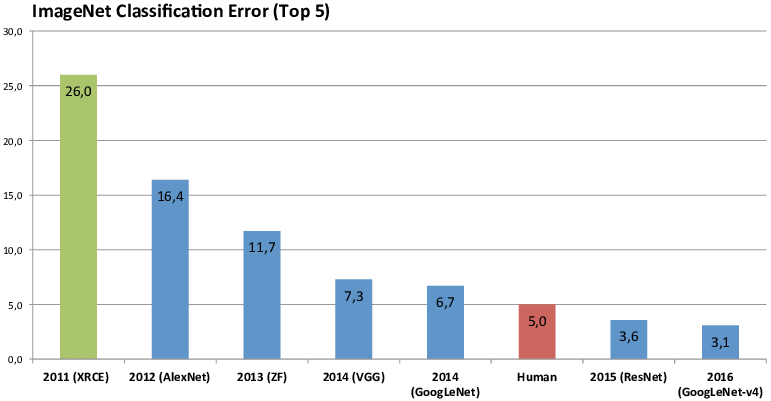
\includegraphics[width=1.0\linewidth]{./img/alexnet.png}
%    \end{figure}
%    \footnotemark{\scriptsize{source: Embedded Vision Alliance (https://www.embedded-vision.com)}}
%\end{frame}

\begin{frame}{Deep Learning and Attention}
    \begin{itemize}
        \item Increasingly more common!
        \item Constantly sets a new SOTA for the tasks attacked
    \end{itemize}
\end{frame}

\begin{frame}{Deep Learning and Attention: Image Captioning}
    \begin{figure}
        \centering
        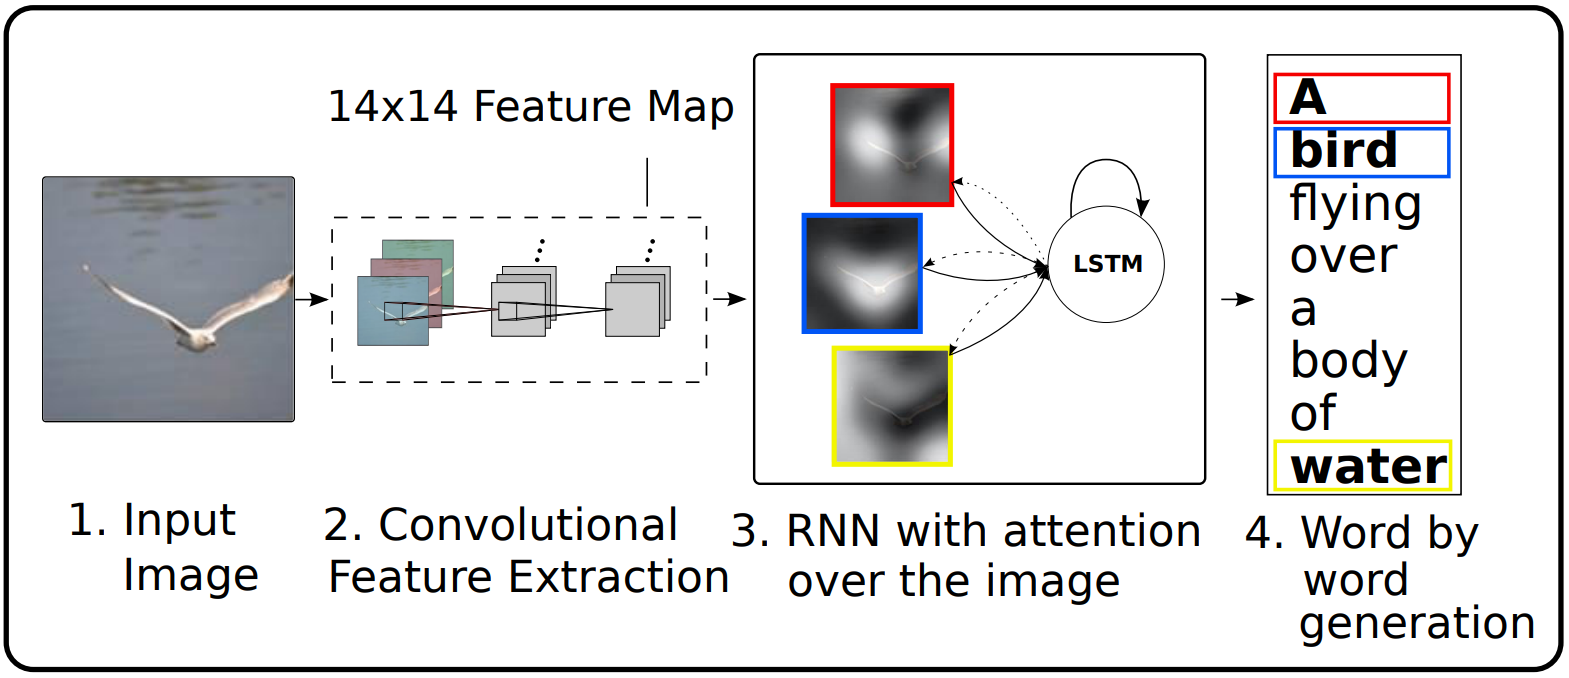
\includegraphics[width=1.0\linewidth]{./img/img_captioning.png}
    \end{figure}
\end{frame}

\begin{frame}{Deep Learning and Attention: rise in interest}
    \begin{figure}
        \centering
        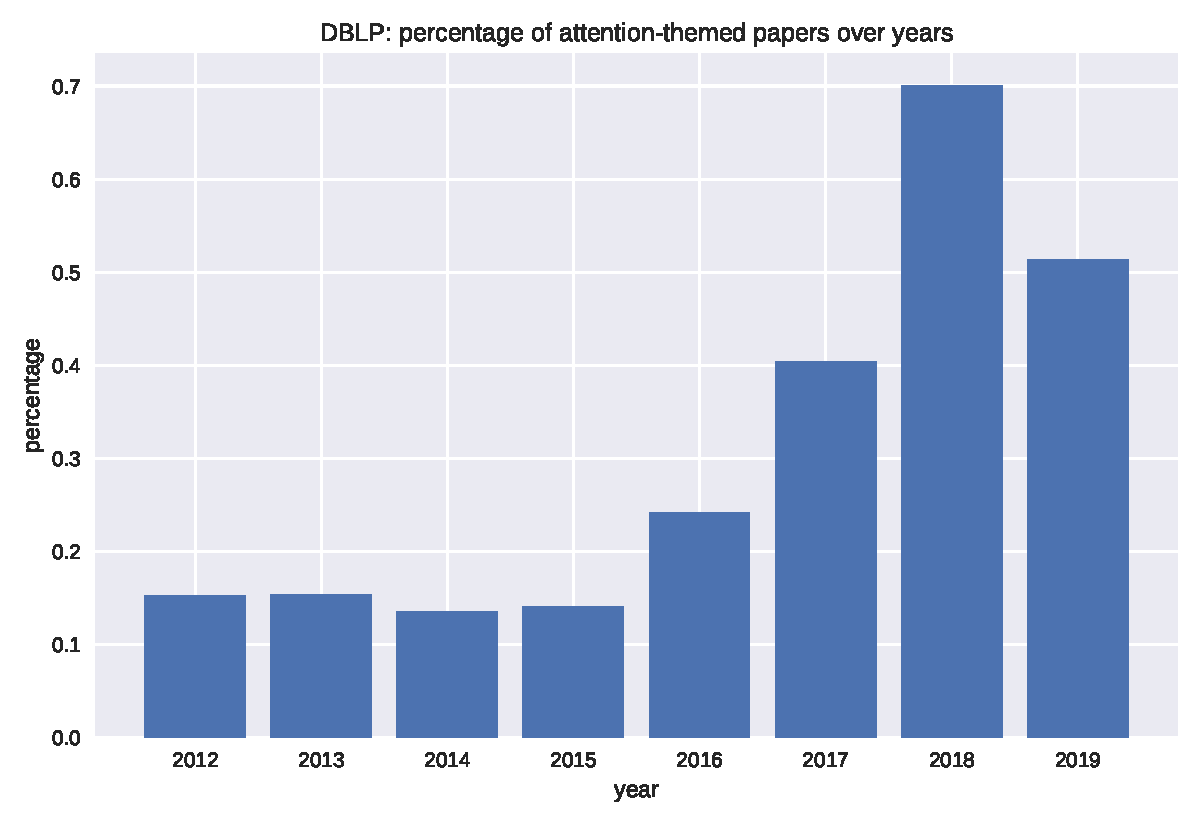
\includegraphics[width=0.9\linewidth]{./img/dblp_att_papers.pdf}
    \end{figure}
    \footnotemark{\scriptsize{source: DBLP (https://dblp.uni-trier.de/)}}
\end{frame}

\begin{frame}{Motivation}
    \begin{itemize}
        \item Many tasks are approached with Deep Learning yet still do not use Attention
        \item There are aspects of Attention still to be explored
        \item We believe it's possible to further generalize Attention for the benefit of Deep Learning
    \end{itemize}
\end{frame}

\begin{frame}{The main contribution}
    \centering
    \textit{
        To establish a framework for applicability of Attention to Deep Learning
        to help guide future development in the area}
\end{frame}

\begin{frame}{Objectives}
    \begin{itemize}
        \item To perform an extensive \textbf{literature review} on the use of Attention
            in modern Deep Learning
        \item To identify \textbf{general elements of Attention} to be applied to Deep Learning
        \item To identify \textbf{specific problems} in different classes
            (robotics, vision, NLP...) with improvement potential through the use of Attention;
        \item To \textbf{propose and implement} one or more solutions based on the findings of the work
            to validate the ideas and evaluate them in an application
    \end{itemize}
\end{frame}

\section{Background}

\begin{frame}{Main concepts of Attention: Functionalities}
    \begin{itemize}
        \item To \textbf{select stimuli} that is relevant
        \item To \textbf{sustain focus} on a specific semantic element for a certain period
        \item To \textbf{guide processing} in a sequential manner that is relevant for a task
        \item To \textbf{orient resources} to new important stimuli
    \end{itemize}
\end{frame}

\begin{frame}{Main concepts of Attention: Bottom-up vs Top-down}
    \begin{itemize}
        \item \textbf{Bottom-up} Attention: involuntarily started and guided by external and conspicuous stimuli
        \item \textbf{Top-down} Attention: cognition and goals voluntarily guide the focus
    \end{itemize}
\end{frame}

% Soft attention pode ser entendido como o processo de ativação neuronal enquanto o hard attention poderia ser tratado como o elemento de tomada de decisão de alocação  (WTA)
\begin{frame}{Main concepts of Attention: Soft vs Hard}
    \begin{itemize}
        \item \textbf{Hard} Attention: \textbf{choice} of items in a possibly non-deterministic manner
            $$z = choice\left(\{x_1, x_2, \ldots, x_n\}\right)$$
        \item \textbf{Soft} Attention: \textbf{weighting} of items in a deterministic manner
            $$z = \sum_{i=1}^{n}{x_i \alpha_i}, \;\;\; 0 \le \sum_{i=1}^{n}{\alpha_i} \le 1$$
    \end{itemize}
\end{frame}

\begin{frame}{Deep Learning}
    \begin{figure}
        \centering
        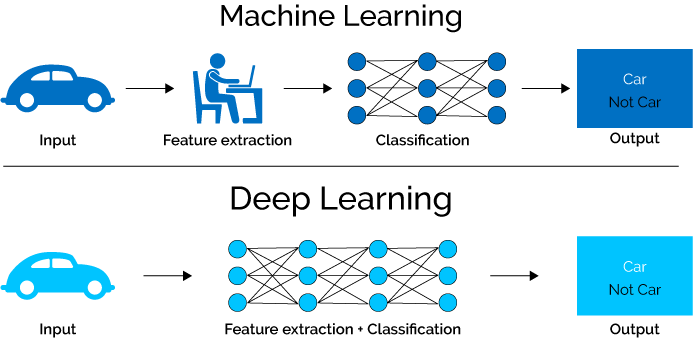
\includegraphics[width=1.0\linewidth]{./img/dl.png}
    \end{figure}
\end{frame}

\begin{frame}{Deep Learning: Deep MLPs}
    \begin{figure}
        \centering
        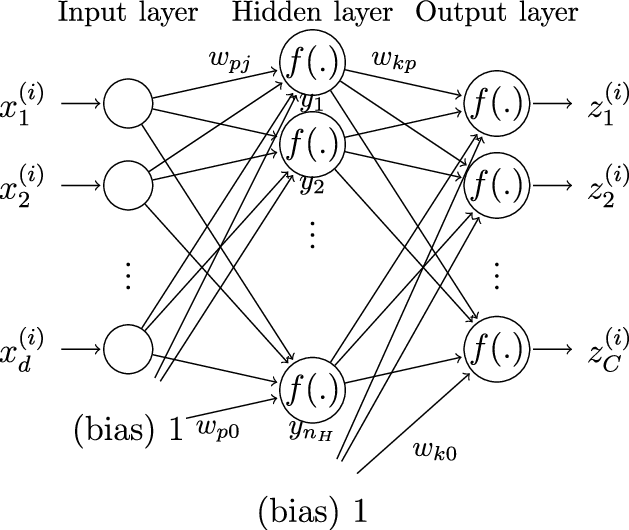
\includegraphics[width=0.7\linewidth]{./img/dl3.png}
    \end{figure}
\end{frame}

\begin{frame}{Deep Learning: ConvNets (CNNs)}
    \begin{figure}
        \centering
        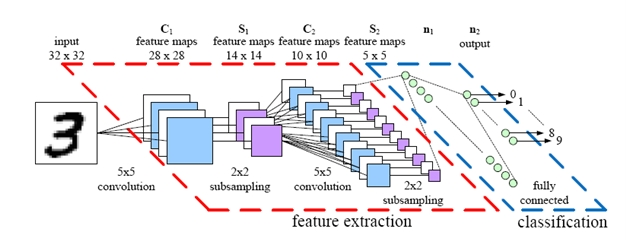
\includegraphics[width=1.0\linewidth]{./img/cnn.png}
    \end{figure}
\end{frame}

\begin{frame}{Deep Learning: Recurrent Neural Networks (RNNs)}
    \begin{figure}
        \centering
        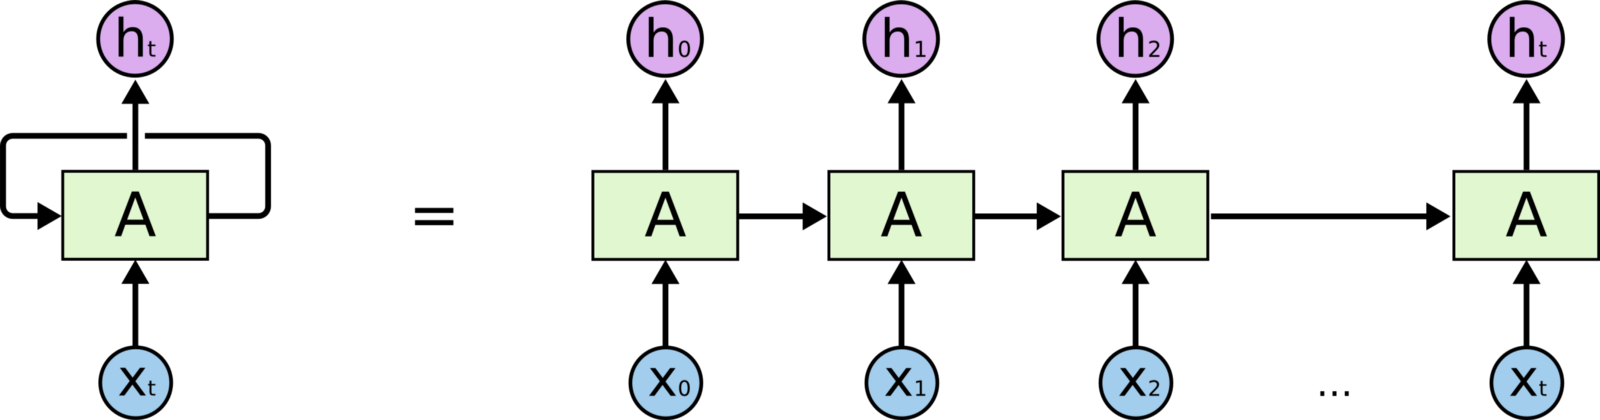
\includegraphics[width=0.9\linewidth]{./img/rnn2.png}
    \end{figure}
\end{frame}

\begin{frame}{Deep Learning: Learning Process}
    \begin{itemize}
        \item The act of learning the appropriate weights of a given model
        \item Usually via \emph{supervised learning}
        \item Usually obtained by the minimization of a differentiable loss function
            $L(y, \hat{y})$, the error between $y$ and $\hat{y}$
        \item Backpropagation plays an essential role in Deep Learning:
        \begin{itemize}
            \item forward-propagation step, which calculates the loss
            \item backpropagation step which adjusts the weights:
    $$\theta_{i+1} = \theta_i - \alpha\frac{\partial{J}}{\partial{\theta}}$$
        \end{itemize}
    \end{itemize}
\end{frame}

%\begin{frame}{Deep Learning models and Attention}
%    \begin{figure}
%        \centering
%        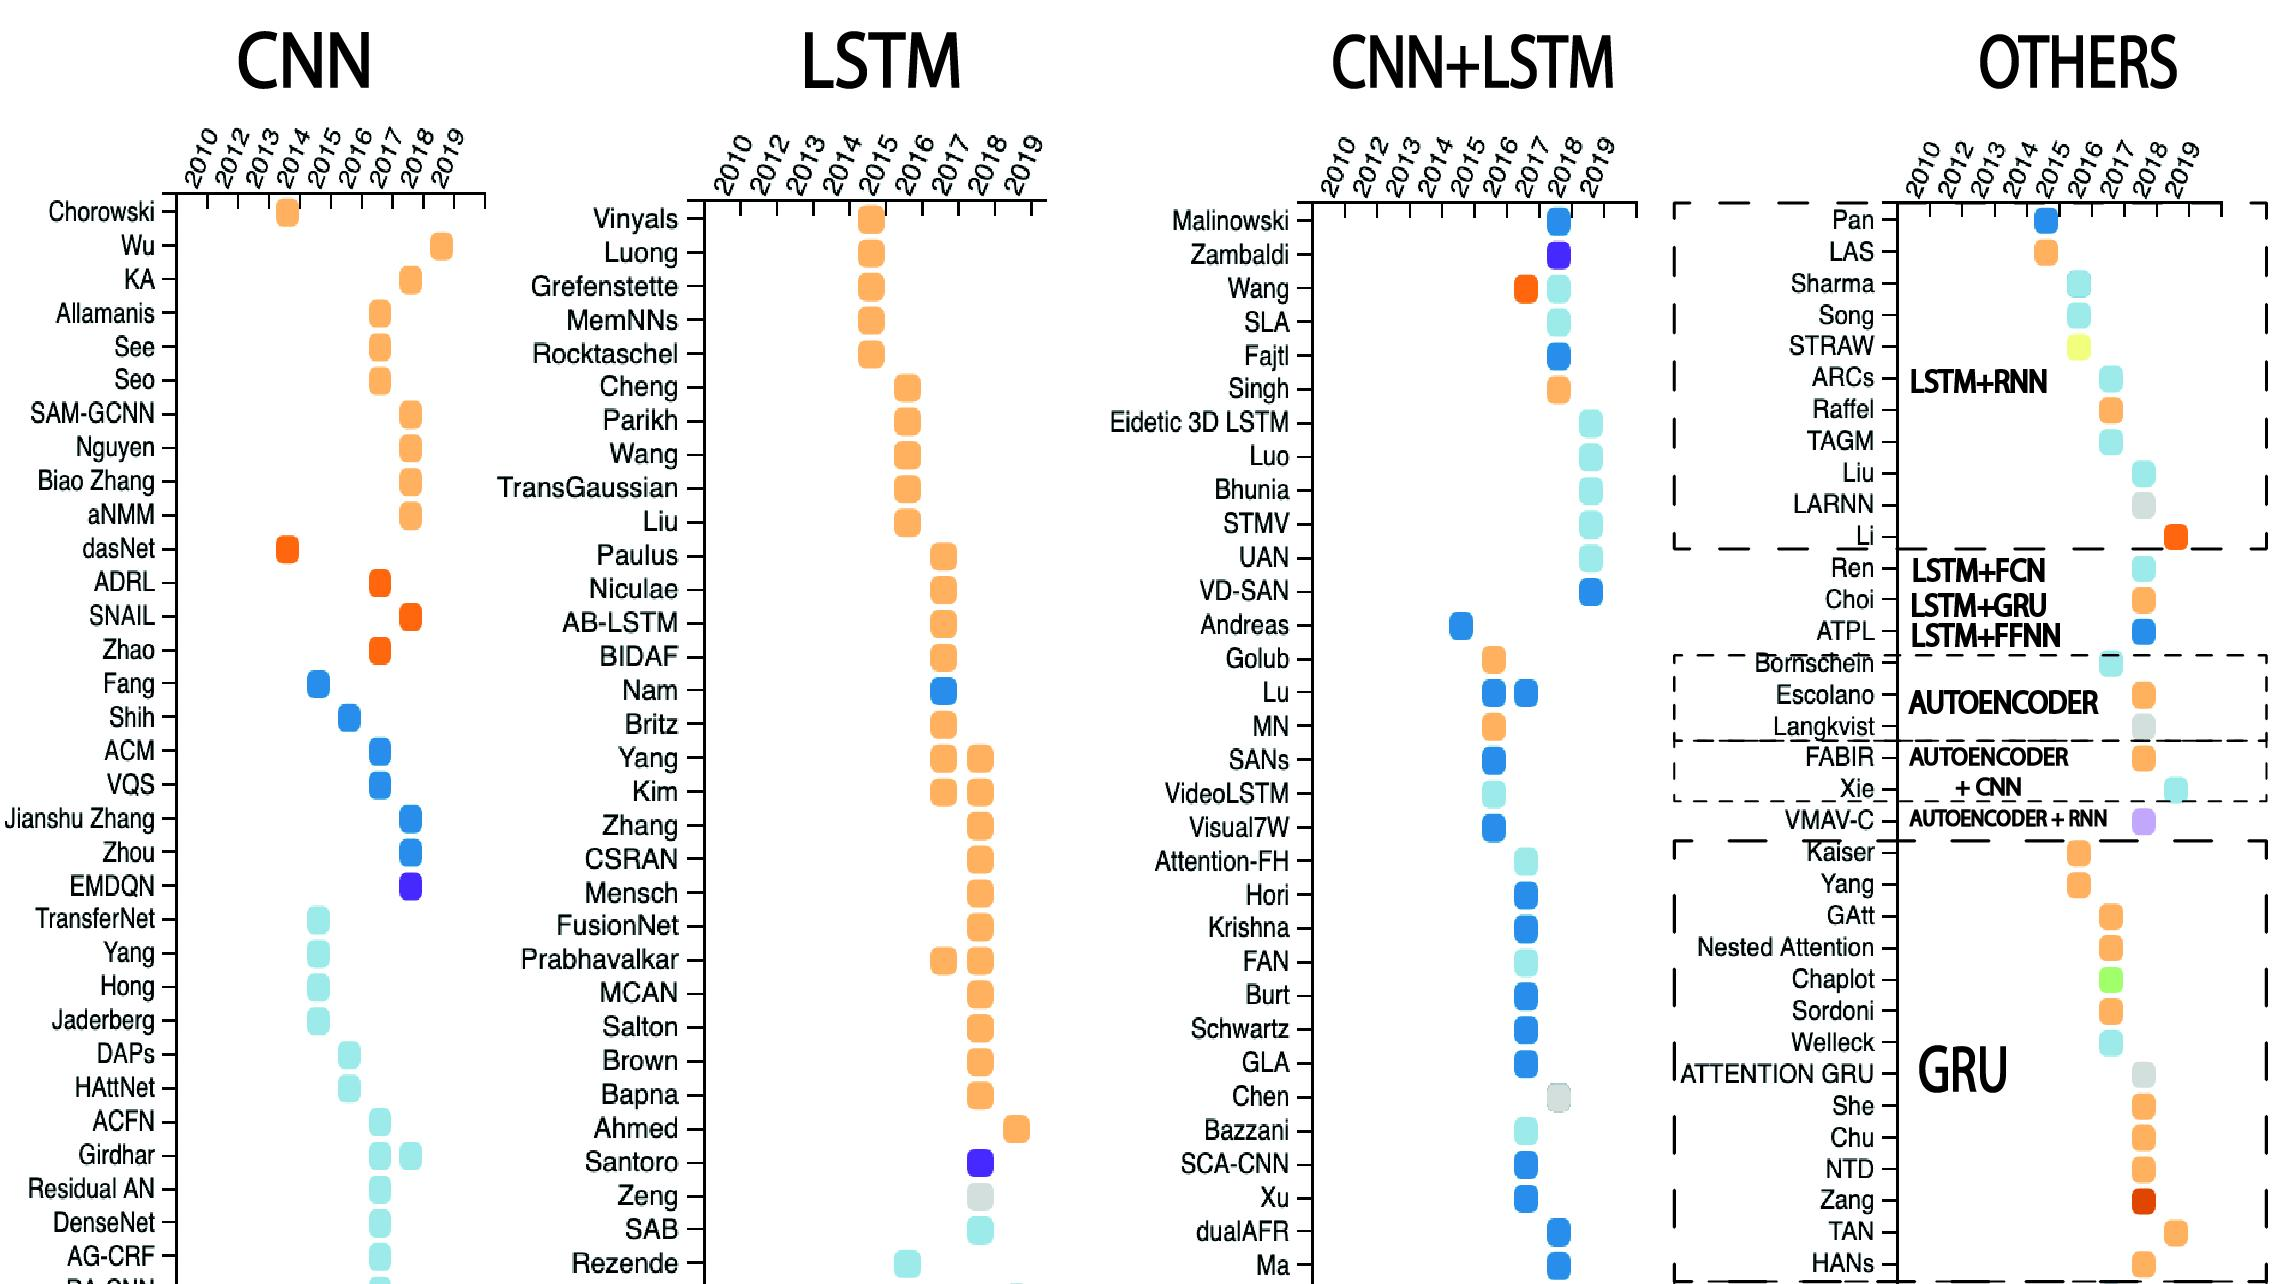
\includegraphics[width=1.0\linewidth]{./img/dl-att-timeline.jpg}
%    \end{figure}
%\end{frame}

%\begin{frame}{Recurrent Attention Model (RAM)}
%    \begin{itemize}
%        \item RNN for general image-related tasks
%        \item At each timestep, extracts a constant-size glimpse of the image
%    \end{itemize}
%\end{frame}

\begin{frame}{Related work: Recurrent Attention Model (RAM)}
    \begin{figure}
        \centering
        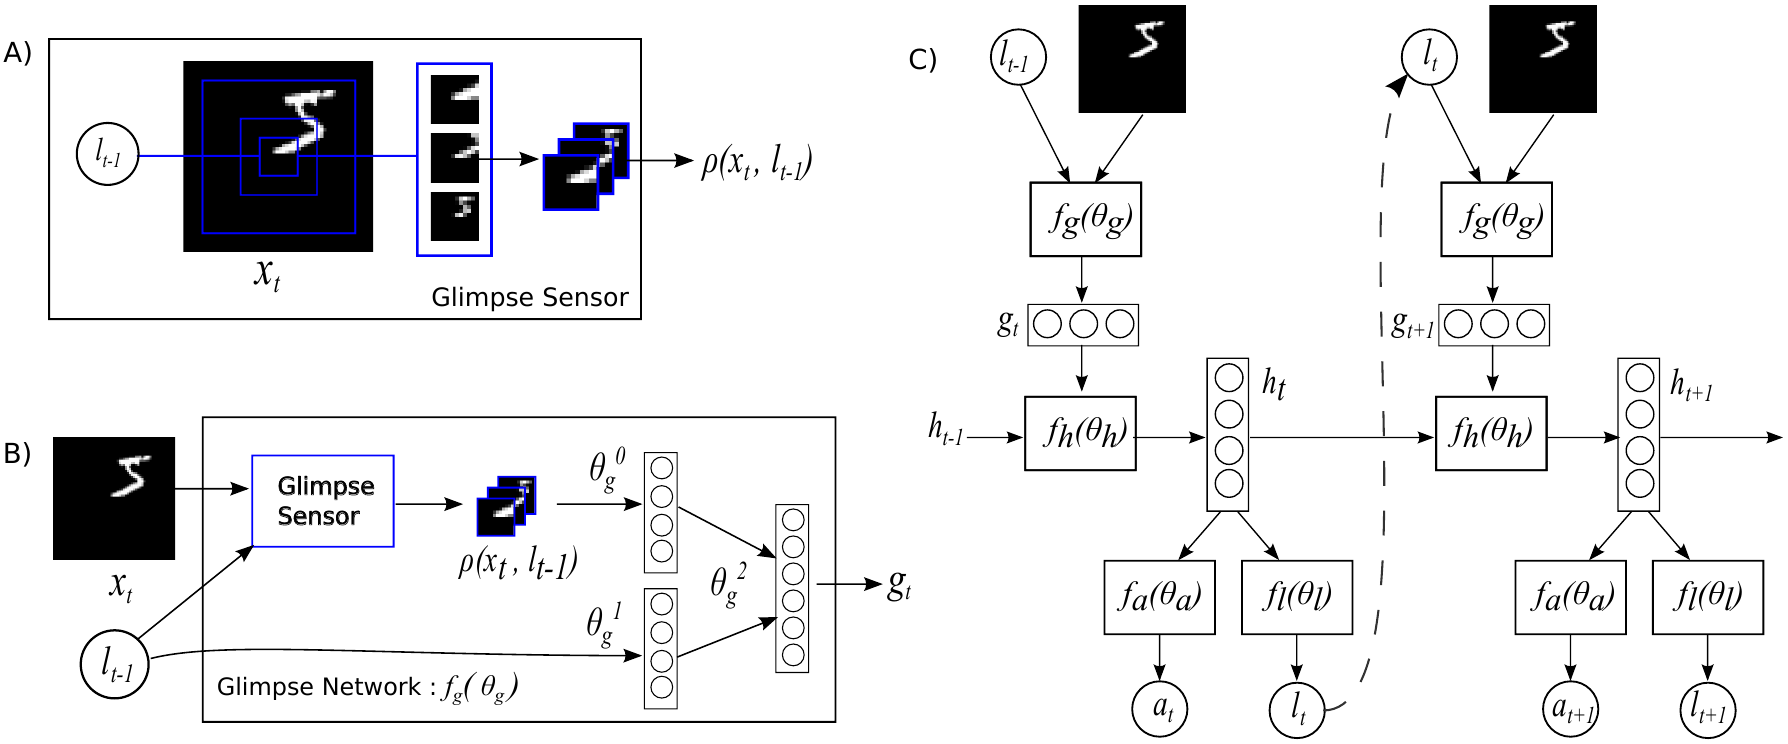
\includegraphics[width=1.0\linewidth]{./img/recurr_model.png}
    \end{figure}
\end{frame}

%\begin{frame}{Attention-based Encoder-Decoder Networks}
%    \begin{itemize}
%        \item Main idea: an attentional module in between encoder and decoder
%        \item Multiple applications with very good results:
%        \begin{itemize}
%            \item \emph{Image Caption Generation}
%            \item \emph{Neural Machine Translation}
%            \item \emph{Neural Speech Recognition}
%        \end{itemize}
%    \end{itemize}
%\end{frame}

%\begin{frame}{Attention-based Encoder-Decoder Networks}
%    \begin{figure}
%        \centering
%        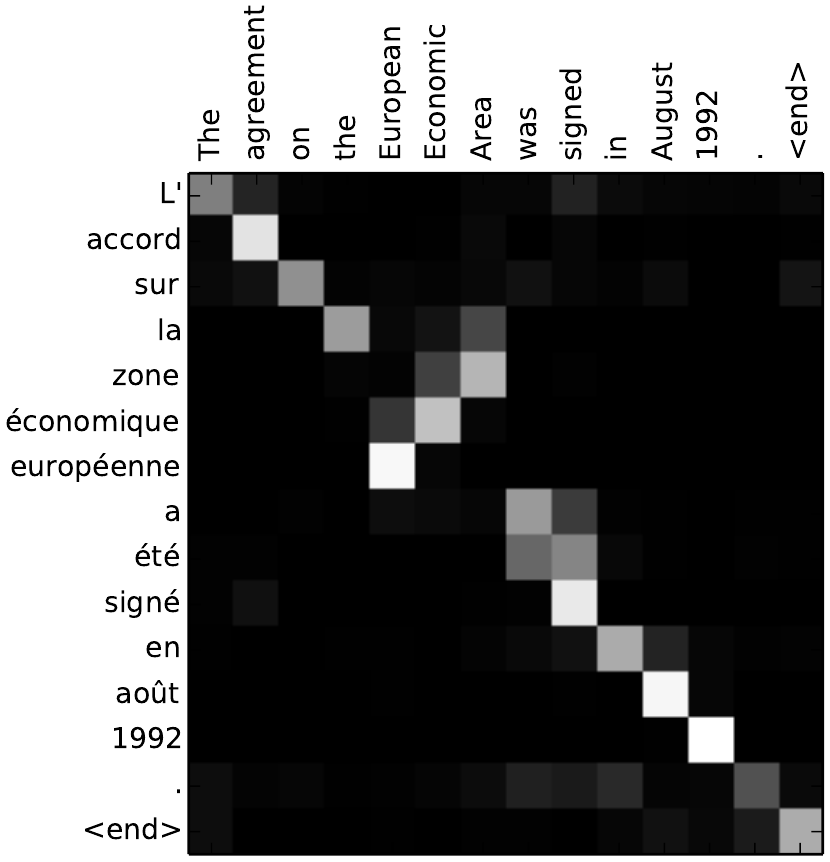
\includegraphics[width=0.6\linewidth]{./img/nt-att.png}
%    \end{figure}
%\end{frame}

%\begin{frame}{Adaptive Computation Time (ACT)}
%    \begin{itemize}
%        \item RNN with dynamic number of sub-steps
%        \item Attention mechanism allocates resources to computation time and data
%    \end{itemize}
%\end{frame}

\begin{frame}{Related work: Adaptive Computation Time (ACT)}
    \begin{figure}
        \centering
        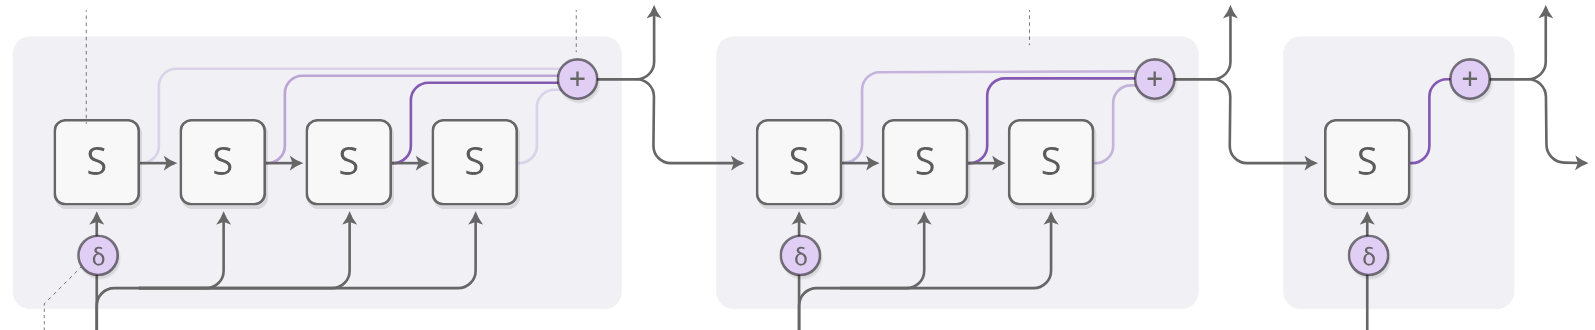
\includegraphics[width=1.0\linewidth]{./img/adaptive_comp.png}
    \end{figure}
\end{frame}

\section{Methodology}

\begin{frame}{Activities}
    \begin{enumerate}
        \item \textbf{A1}: Literature Review
        \begin{itemize}
            \item \textbf{A1.1}: Theoretical framework for Attention
            \item \textbf{A1.2}: Elaboration of survey
            \item \textbf{A1.2}: Survey article writing
        \end{itemize}
        \item \textbf{A2}: Proposal of an Attention framework for Deep Learning
        \begin{itemize}
            \item \textbf{A2.1}: Establishment of Attention components for specific Deep Learning domains
        \end{itemize}
        \item \textbf{A3}: Validation of framework
        \begin{itemize}
            \item \textbf{A3.1}: Arrangement of experiments
            \item \textbf{A3.2}: Execution of experiments
            \item \textbf{A3.3}: Evaluation of experimental results
            \item \textbf{A3.4}: Experiments article writing
        \end{itemize}
        \item \textbf{A0}: Masters activities
        \begin{itemize}
            \item \textbf{A0.1}: Course's requirement fulfillment
            \item \textbf{A0.2}: Qualification Exam
            \item \textbf{A0.3}: Masters dissertation
            \item \textbf{A0.4}: Defense of masters dissertation
        \end{itemize}
    \end{enumerate}
\end{frame}

\begin{frame}{Schedule}
    \begin{table}[H]
    \centering
    \caption{\small Project schedule.}
    \tiny
    \begin{tabular}{|c|c|c|c|c|c|c|c|c|c|c|c|c|c|}
        \hline
        \textbf{Activity} & \multicolumn{12}{|c|}{\textbf{2019}}\\
        \hline
                      & Jan & Feb & Mar & Apr & May & Jun & Jul & Aug & Sep & Oct & Nov & Dec\\
        \hline
        \textbf{A1.2} & $*$ & $*$ & $*$ & $*$ & $*$ & $*$ & $*$ &     &     &     &     &     \\
        \hline
        \textbf{A0.2} &     &     &     &     & $*$ &     &     &     &     &     &     &     \\
        \hline
        \textbf{A1.3} &     &     &     &     &     &     & $*$ &     &     &     &     &     \\
        \hline
        \textbf{A2.1} &     &     &     &     &     &     & $*$ &     &     &     &     &     \\
        \hline
        \textbf{A3.1} &     &     &     &     &     &     &     & $*$ &     &     &     &     \\
        \hline
        \textbf{A3.2} &     &     &     &     &     &     &     & $*$ & $*$ & $*$ & $*$ &     \\
        \hline
        \textbf{A3.3} &     &     &     &     &     &     &     &     &     &     & $*$ &     \\
        \hline
        \textbf{A3.4} &     &     &     &     &     &     &     &     &     &     & $*$ &     \\
        \hline
        \textbf{A0.3} &     &     &     &     &     &     &     &     &     & $*$ & $*$ & $*$ \\
        \hline
        \textbf{A0.4} &     &     &     &     &     &     &     &     &     &     &     & $*$ \\
        \hline
    \end{tabular}
    \label{table:sched}
    \end{table}
\end{frame}

\section{Work so far}

\begin{frame}{Theoretical Framework for Attention}
    Two main parts:
    \begin{enumerate}
        \item A \textbf{definition} of Attention (\emph{what} is Attention?)
        \item A \textbf{model} of Attention (\emph{how} does attention emerge?)
    \end{enumerate}
\end{frame}

\begin{frame}{Theoretical Framework for Attention: why?}
    \begin{itemize}
        \item We need a \emph{precisely defined} basis to be work upon for:
        \begin{itemize}
            \item The analysis of papers in the literature review
            \item The solutions and models proposed in the future
            \item ...
        \end{itemize}
    \end{itemize}
\end{frame}

\begin{frame}{A definition of ``Attention''}
    \begin{itemize}
        \item \textbf{Goal}: define a set of \emph{entities of interest} and the phenomenon of Attention in terms of its \emph{functionalities} and how it relates to the entities.
        \item \textbf{Why this goal?}
            \begin{itemize}
                \item There are multiple (conflicting) definitions of what ``Attention'' is
                \item We need to postulate a \emph{precise definition} in which all of our work will be based upon
            \end{itemize}
    \end{itemize}
\end{frame}

\begin{frame}{A definition of ``Attention'': entities}
    \begin{itemize}
        \item\textbf{Data:} information, stimuli.
        \item\textbf{Program:} algorithm, sequence of computer (or mental) operations.
        \item\textbf{Process:} the execution of a program on a specific data instance.
        \item\textbf{Computer:} the executor of processes, the brain.
        \item\textbf{Resource:} when not specified, we mean computational resources, e.g., CPU time.
        \item\textbf{Time:} the flow of time.
        \item\textbf{World:} the external environment.
        \item\textbf{Agent:} the actor in the world.
        \item\textbf{Actions:} the interaction of the agent with the world.
        \item\textbf{Goals:} the ends, objectives to be met.
    \end{itemize}
\end{frame}

\begin{frame}{A definition of ``Attention''}
    \centering
    \textbf{Data}, \textbf{programs} and \textbf{processes} are virtually \textbf{infinite}.
    Computational \textbf{resources} and \textbf{actions} are finite.

    \textbf{Attention} is \textbf{the system for allocating resources to processes}.

    In other words, \textbf{attention} is the entity in \textbf{agent} that, given \textbf{context} and a set of \textbf{processes},
    \textbf{allocates} \textbf{resources} to execute each of them in order to \textbf{produce} \textbf{outputs} in form of \textbf{data} and \textbf{actions} in a \textbf{correct sequential manner} and in \textbf{sensible time} in order to reach \textbf{goals}.
\end{frame}

\begin{frame}{A model for Attention}
    \begin{itemize}
        \item Proposal: to model Attention as a phenomenon that emerges from the use of \textbf{attention modules} in a system
    \end{itemize}
\end{frame}

\begin{frame}{A model for Attention}
    \begin{figure}
        \centering
        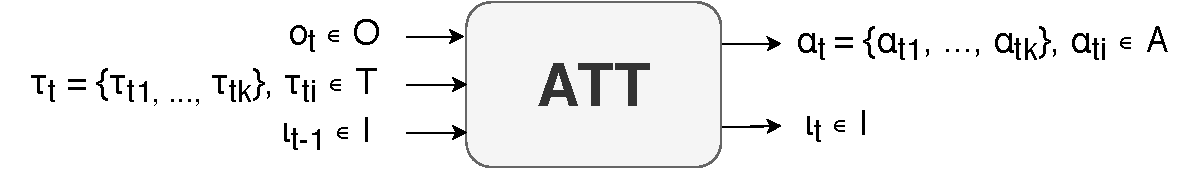
\includegraphics[width=1.0\linewidth]{./img/alt_att_block.pdf}
    \end{figure}
\end{frame}

\begin{frame}{A model for Attention}
    \begin{figure}
        \centering
        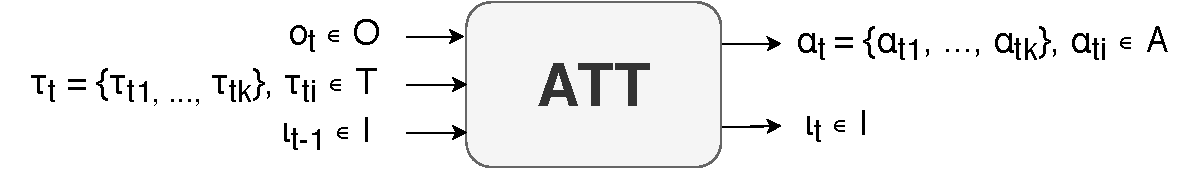
\includegraphics[width=1.0\linewidth]{./img/alt_att_block.pdf}
    \end{figure}
    At each time step $t$, the module receives as \emph{input}:
    \begin{itemize}
        \item Current \emph{outer state} $o_t \in O$, where $O$ is the \emph{outer state set}
        \item Group of \emph{focus targets} $\tau_t = \{\tau_{t1}, \ldots, \tau_{tk}\}, \tau_{ti} \in T$, where $T$ is the \emph{focus target set}
        \item Past \emph{inner state} $\iota_{t-1} \in I$, where $I$ is the \emph{inner state set}
    \end{itemize}

    The module produces as \emph{output} (as a function of both inputs):
    \begin{itemize}
        \item Current \emph{inner state} $\iota_t \in I$
        \item Current \emph{focus output} $\alpha_t = \{\alpha_{t1}, \ldots, \alpha_{tk}\}, \alpha_{ti} \in A$,
            where $A$ is the \emph{focus output set}
    \end{itemize}
\end{frame}

\begin{frame}{A model for Attention: Focus output}
    \begin{itemize}
        \item The main element of the module
        \item Can be used to allocate \emph{finite resources} to a set of candidate targets by giving them an importance score
        \item Each element $\alpha_{tk}$ is respective to a target element $\tau_{tk}$.
        \item Target elements ($\tau \in T$) may effectively be \emph{programs} (tasks) or \emph{data}.
    \end{itemize}
\end{frame}

\begin{frame}{A model for Attention: Soft and Hard Attention}
    \begin{itemize}
        \item \textbf{Soft Attention:}
            $A = [0, 1]$, with $0 \le \sum_{i=1}^{k} \alpha_{ti} \le 1$
        \item \textbf{Hard Attention:}
            $A = \{0, 1\}$, with $0 \le \sum_{i=1}^{k} \alpha_{ti} \le M$ and $0 \le M \le |\tau_t|$
    \end{itemize}
\end{frame}

\begin{frame}{A model for Attention: Bottom-up and Top-down Attention}
    Depends on the \emph{location} of the module:
    \begin{itemize}
        \item \textbf{Bottom-up}: module connected to external stimulus features (e.g. images)
        \item \textbf{Top-down}: module connected to internal/context information
    \end{itemize}
\end{frame}

\begin{frame}{A model for Attention: Example}
    \begin{figure}[H]
        \centering
        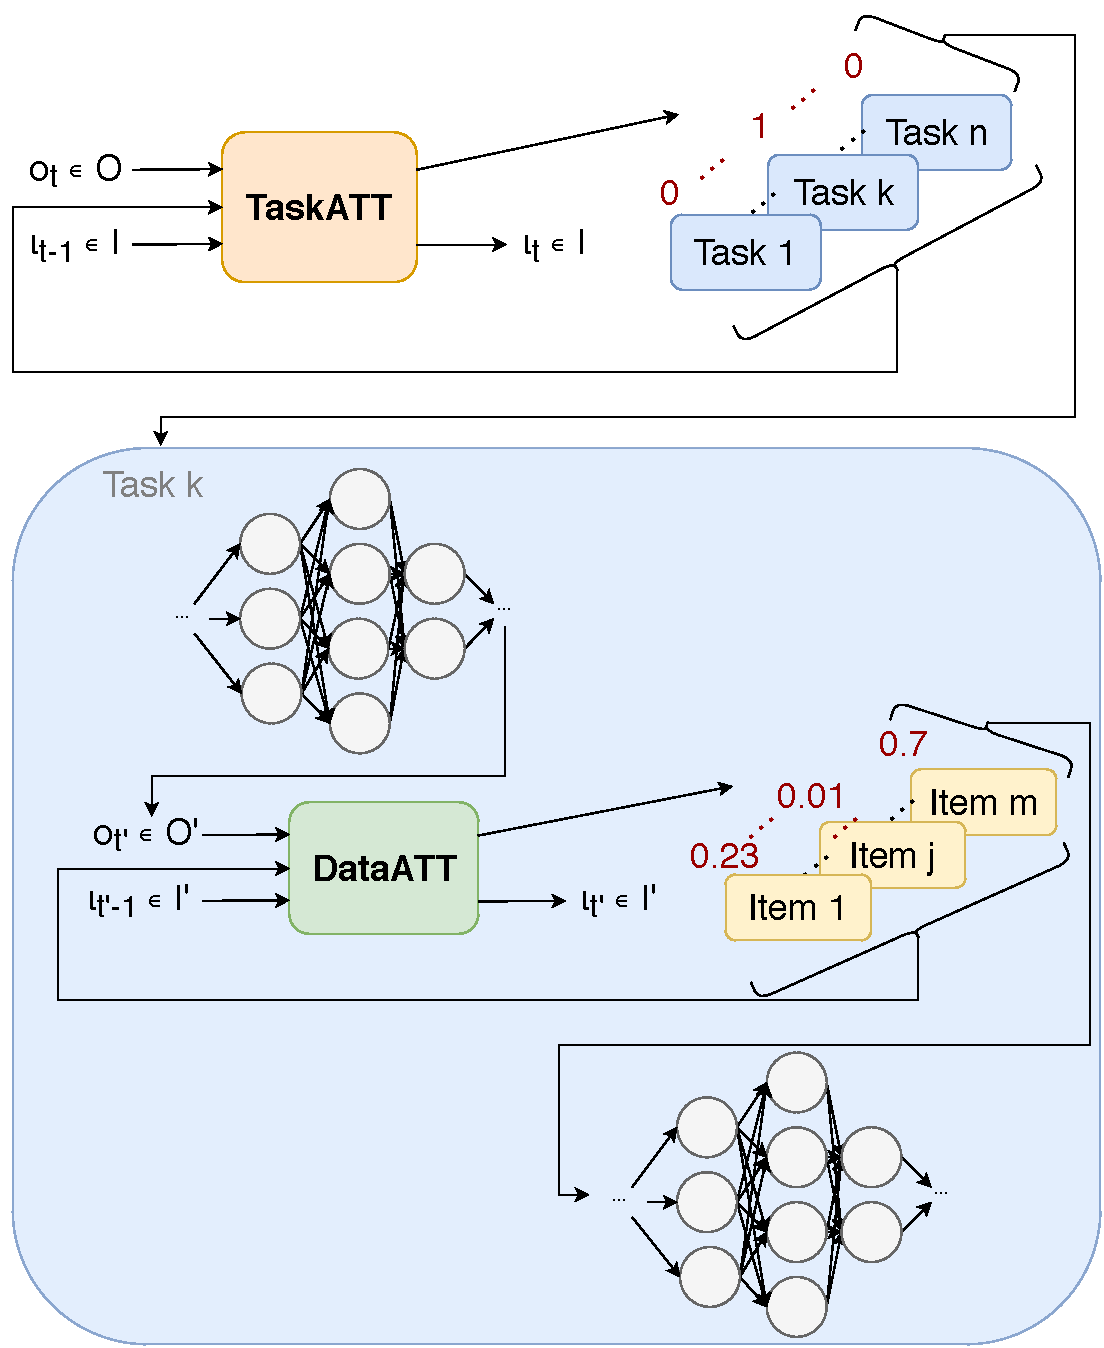
\includegraphics[width=0.6\linewidth]{./img/att_blocks_example.pdf}
    \end{figure}
\end{frame}

\begin{frame}{Validating the model for Attention: Image Captioning}
    \begin{itemize}
        \item Work is among the first to propose using attention to image caption generation
        \item Encoding of the input image is represented as a set of vectors - each respective to a certain spatial region of the image -
        \item The attentional component gives weights to each vector at each step to produce another vector to be used in further computations
    \end{itemize}
\end{frame}

\begin{frame}{Validating the model for Attention: Image Captioning}
    \begin{figure}[H]
        \centering
        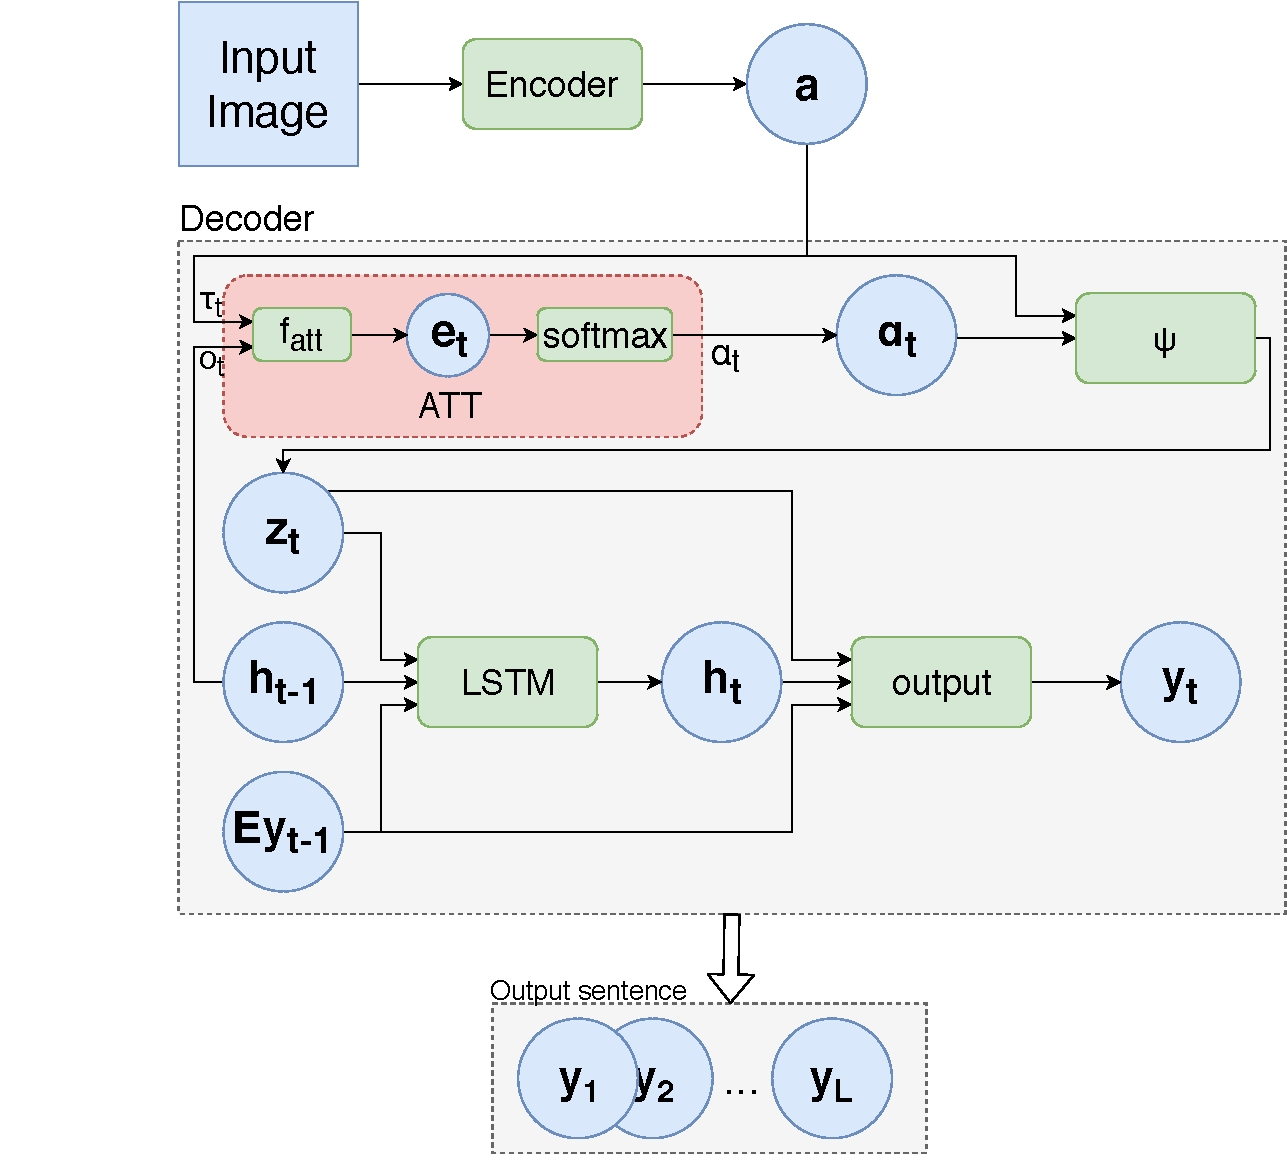
\includegraphics[width=0.6\linewidth]{./img/captioning.pdf}
    \label{fig:cap}
\end{figure}

\end{frame}

\begin{frame}{Validating the model for Attention: Adaptive Computation Time}
    \begin{itemize}
        \item Work proposes a RNN with dynamically variable number of computation steps
        \item Uses attention to allocate processing ``budget'' and selection of data
    \end{itemize}
\end{frame}

\begin{frame}{Validating the model for Attention: Adaptive Computation Time}
    \begin{figure}[H]
        \centering
        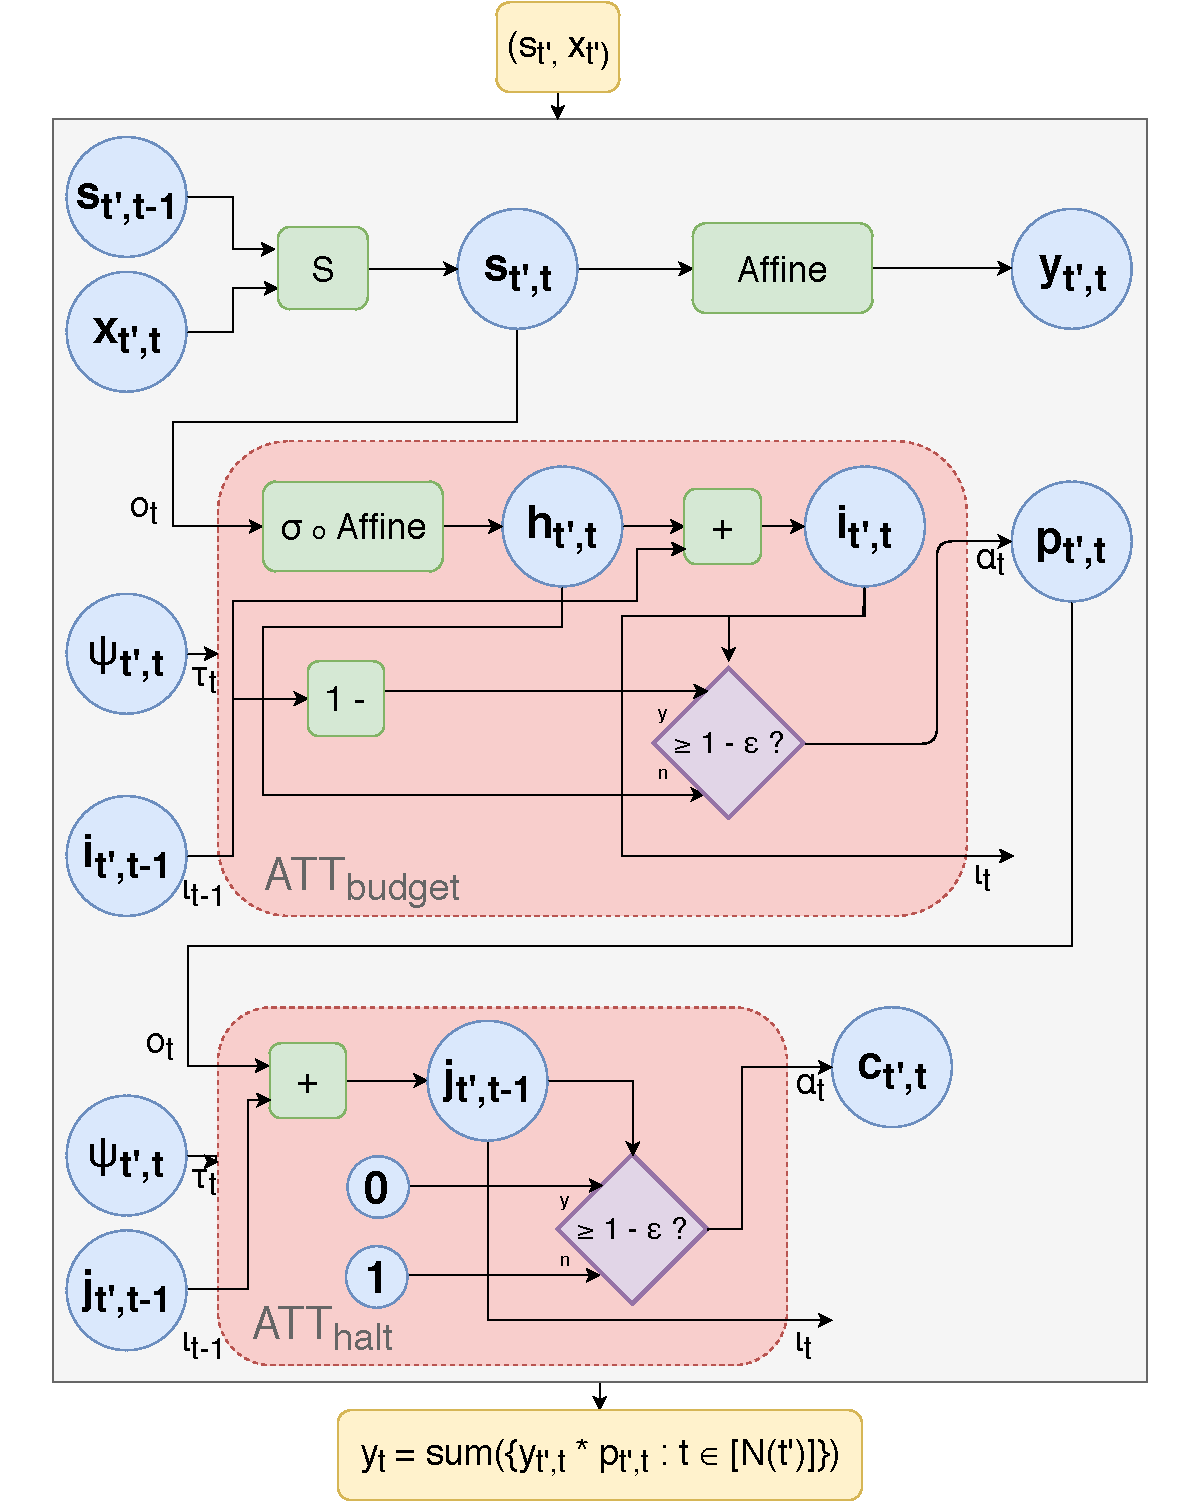
\includegraphics[width=0.55\linewidth]{./img/act.pdf}
    \end{figure}
\end{frame}

\begin{frame}{Validating the model for Attention: Adaptive Computation Time}
    Proposed model can be thought of as having two attention modules:
    \begin{itemize}
        \item \textbf{$ATT_{budget}$}:
            \begin{itemize}
                \item Computes the value $0 \le p_{t',t} \le 1$ to be spent at a given sub-step
                \item \emph{Focus output} $p_{t',t}$, represents values to be consumed from the budget and
                    an importance weight for the final output $y_t$.
            \end{itemize}
        \item \textbf{$ATT_{halt}$}:
            \begin{itemize}
                \item Computes the \emph{continue} value $c_{t',t} \in \{0, 1\}$
            \end{itemize}
    \end{itemize}
    \textbf{The emergent effect}:
    the model can \emph{allocate resources to processes} both by
    \emph{choosing the data} and \emph{amount of computation time to use}
\end{frame}

\begin{frame}{Validating the model for Attention: Recurrent Visual Attention}
    \begin{itemize}
        \item The work proposes a general recurrent model that uses visual attention at each step
        \item Model selects a retina-like representation of a portion of the input image
        \item An arbitrary action $a_t$ can be executed to possibly alter the environment
    \end{itemize}
\end{frame}

\begin{frame}{Validating the model for Attention: Recurrent Visual Attention}
    \begin{figure}[H]
        \centering
        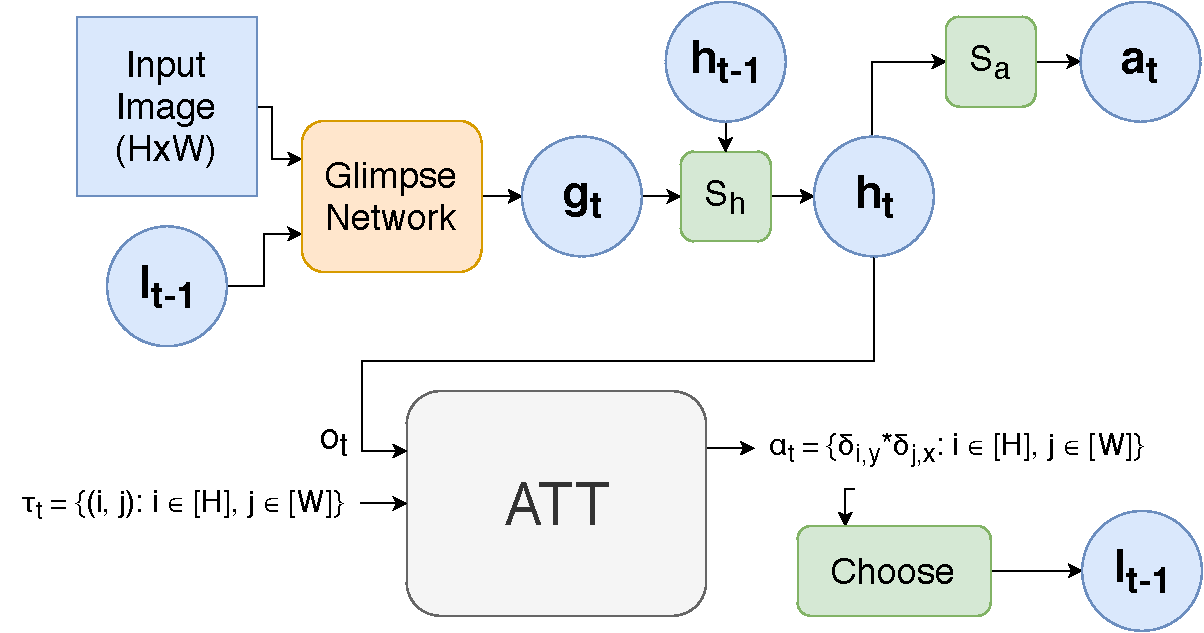
\includegraphics[width=0.9\linewidth]{./img/ram.pdf}
    \end{figure}
\end{frame}

\begin{frame}{Survey}
    \begin{itemize}
        \item \textbf{Main goal}: to perform a \textbf{broad analysis of recent works} that propose attention-based solutions \textbf{under the perspective of our theoretical framework}
    \end{itemize}
\end{frame}

\begin{frame}{Survey: collection of relevant works}
\begin{itemize}
    \item \textbf{Publication date range}: from 2014 to 2019
    \item \textbf{Databases searched}:
    \begin{itemize}
        \item \textbf{arXiv} - \url{https://arxiv.org/}
        \item \textbf{DeepMind} - \url{https://deepmind.com/research/publications/}
        \item \textbf{Google AI} - \url{https://ai.google/research/pubs/}
        \item \textbf{OpenAI} - \url{https://openai.com/research/#publications}
        \item \textbf{NIPS} - \url{https://nips.cc/}
        \item \textbf{ICML} - \url{https://icml.cc/}
        \item \textbf{CVPR} - \url{http://cvpr2018.thecvf.com/}
        \item ...
    \end{itemize}
    \item \textbf{Terms (in title or abstract)}: ``attention'',
        ``attentive'' or ``attentional''
    \item The \textbf{relevance} of each work was confirmed upon the reading of the abstract
    \item As a result, we collected around \textbf{300 papers}
    \item We used \emph{Zotero} and grouped works based on application domain, architectures...
\end{itemize}
\end{frame}

\begin{frame}{Survey: Visualization of papers data}
    \begin{itemize}
        \item Some visualizations were generated for insights
        \item Analysis include:
        \begin{itemize}
            \item Citations graph (authors and works)
            \item Abstract/title word frequencies
            \item Frequency of attention-themed papers over the years
        \end{itemize}
    \end{itemize}
\end{frame}

\begin{frame}{Survey: Data visualization - works citations graph}
    \begin{figure}
    \begin{center}
        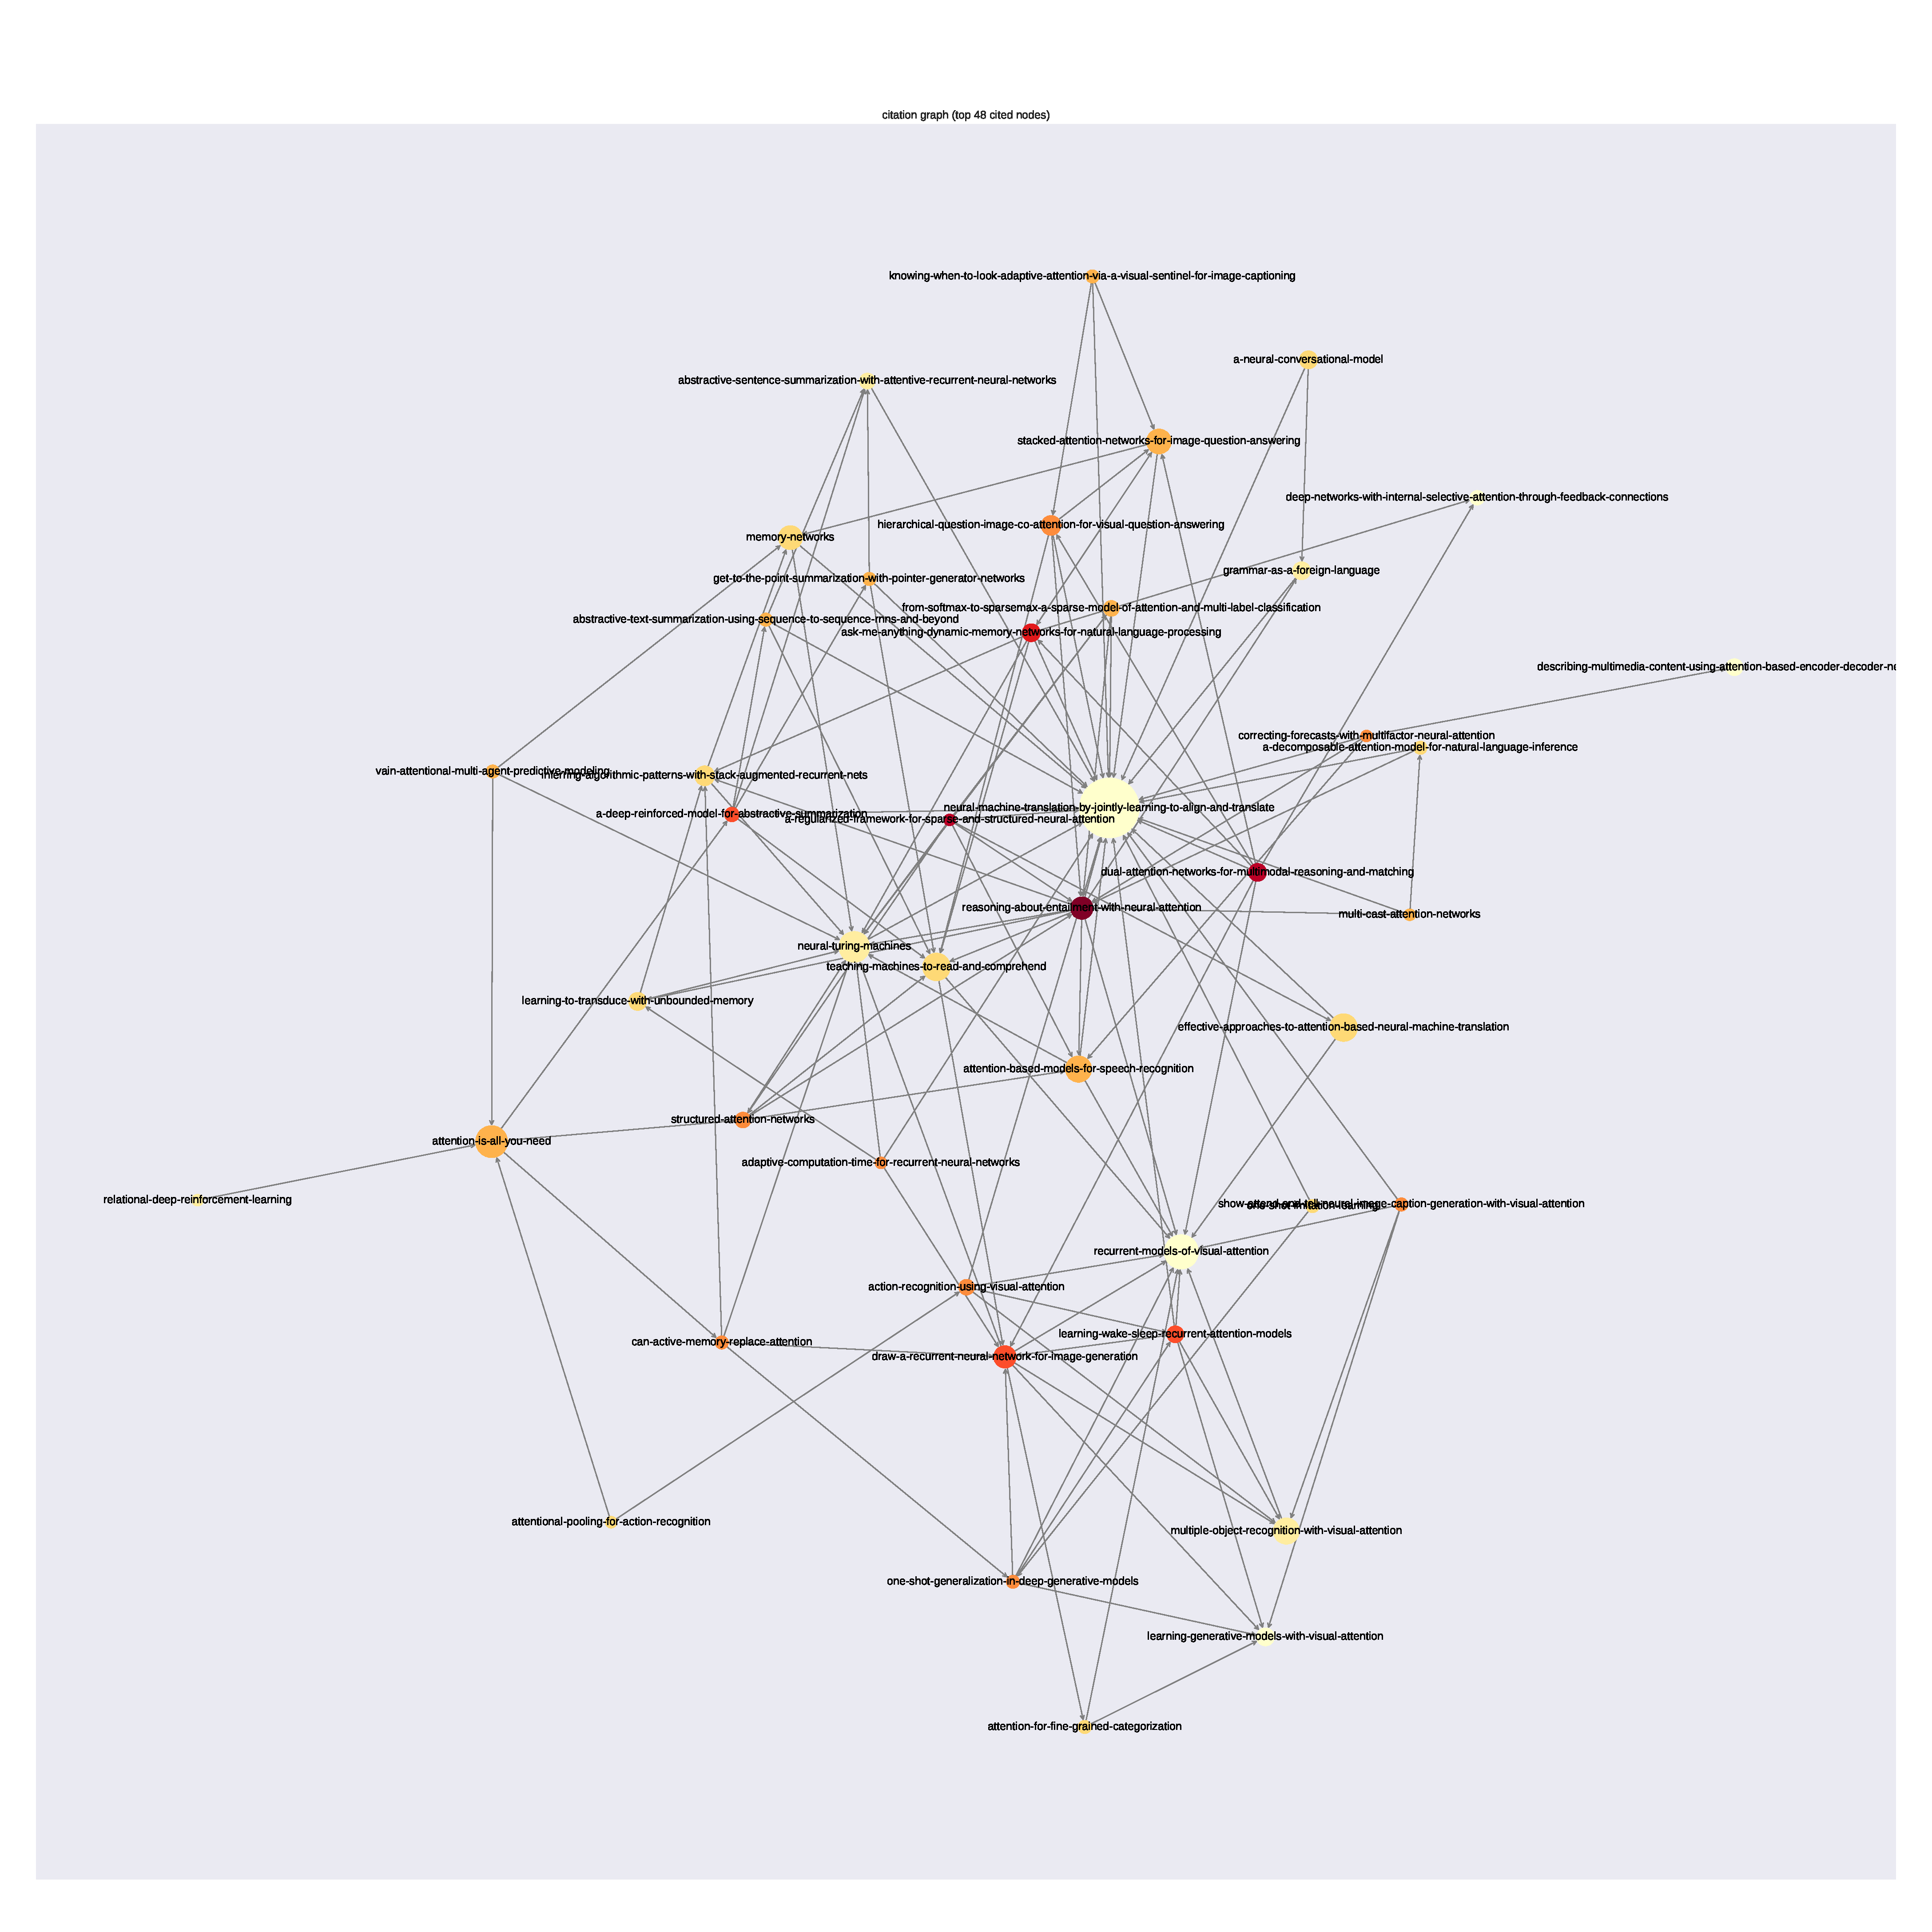
\includegraphics[width=0.8\linewidth]{./img/titles-graph.pdf}
    \end{center}
    \end{figure}
\end{frame}

\begin{frame}{Survey: Data visualization - frequency of terms in abstract}
    \begin{figure}
    \begin{center}
        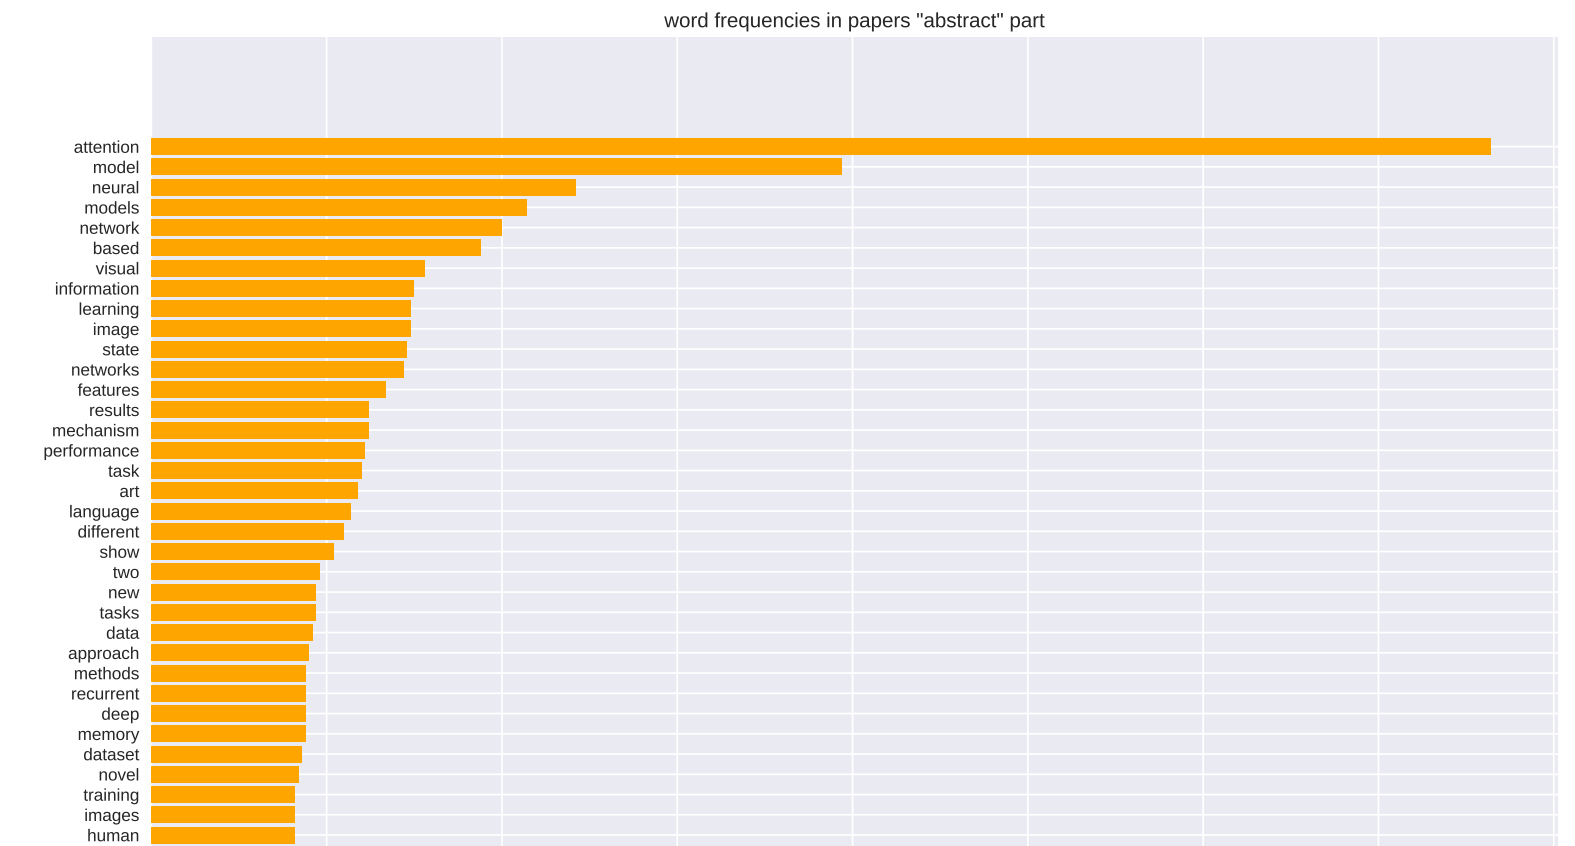
\includegraphics[width=1.0\linewidth]{./img/words_freqs_abs.png}
    \end{center}
    \end{figure}
\end{frame}

\begin{frame}{Survey: Data visualization - frequency of papers over years}
    \begin{figure}
    \begin{center}
        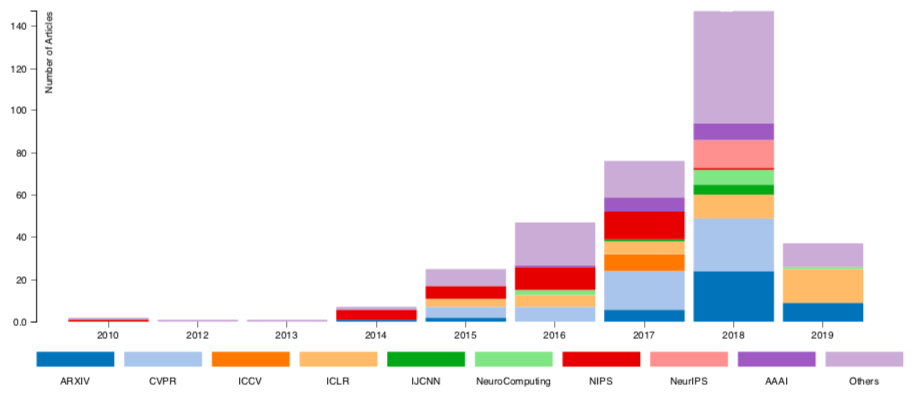
\includegraphics[width=1.0\linewidth]{./img/n_articles.png}
    \end{center}
    \end{figure}
\end{frame}

\begin{frame}{Survey: paper relevance analysis}
    \begin{itemize}
        \item Goal: to assess the relevance and problem domain of each work
        \item To each work, we attributed the citation count, domains and an impact score ranging from 1 to 5
        \item Score was assessed in a quick and rough manner via the abstract of each work:
            \begin{itemize}
                \item How innovative is the proposed model(s) of the work?
                \item How general is the proposed model(s)?
                \item Does the proposed model(s) archives/surpasses state-of-the-art in some task?
                \item Is attention a central component to the results of the work?
            \end{itemize}
    \end{itemize}
\end{frame}

\begin{frame}{Survey: Reading and summarization of works}
    \begin{itemize}
        \item Goal: Obtain a summarization and deep analysis for each paper in the collection
            (in order of relevance, from highest to lowest)
        \item A summary template was formulated and summaries were generated for some works.
        \item The main and longest step of the survey
        \item We may further refine our theoretical framework and to guide the reading of future papers as we read those papers
        \item Survey has shown so far that the use of attention in Deep Learning has indeed provided improvements in basically all
subfields of Deep Learning.
    \end{itemize}
\end{frame}

\begin{frame}{Next Steps}
    \begin{itemize}
        \item Survey:
        \begin{itemize}
            \item Finish papers analysis
            \item Refine theoretical framework
            \item Write and publish survey paper
        \end{itemize}
    \item With the framework and findings of the survey, choose a problem domain and task to attack with an attention-based model. Probably a robotics problem using Reinforcement Learning
    \end{itemize}
\end{frame}

\section{Thank you}

\section{Questions}

%\begin{frame}{References}
%\end{frame}

\end{document}
